\documentclass[a4paper, 11pt]{article}
\usepackage{comment} % enables the use of multi-line comments (\ifx \fi) 
\usepackage{lipsum} %This package just generates Lorem Ipsum filler text. 
\usepackage{fullpage} % changes the margin
\usepackage{graphicx}
\usepackage{subfig}
\graphicspath{ {report/} }

\begin{document}
\noindent
\large\textbf{EIASR report} \hfill \textbf{Szymon Michalski} \\
\normalsize 17Z \hfill Fruits and Vegetables Classifier\\


\section*{Task Description}
The project is to create classifier for fruits and vegetables. 
There is given subset of fruits and vegetables: orange, apple, watermelon, cauliflower, broccoli. Additionally there is one more class describing not known objects.
Classifier will give an answer of the type of the object on the input and will also be able to tell if it is an object not from the given list of learned objects.

\section*{Proposed solution}
In order to solve the given problem the following solution was proposed:
Features will be extracted from images via SIFT algorithm. Later features will be added to Bag of Words. Finally images will be classified using Support Vector Machine.

\section*{Final program}
The proposed solution was implemented exactly as it was proposed in the preliminary report. From the given subset of fruits watermelon was removed, because this class was completely not recognized correctly. For the other classes it is visible that classifier works, even though the accuracy is far from perfection.

\section*{Testing Images Selection}
Due to lack of prepared dataset of already tagged fruits and vegetables imaged, images were gathered from www.image-net.org and www.google.com and thoroughly checked. Then they were divided into six classes: orange, apple, cauliflower, broccoli, other. In total only 307 images were qualified to be train data, and 146 images for test purposes. Most of the data is the class "other" which were taken from MIT Objects 101 dataset.
\textbf{Number of images per category}:
Train data:
'apple': 74, 'cauliflower': 60, 'broccoli': 38, 'orange': 51, 'other': 84

\textbf{Test data:}
'apple': 20, 'cauliflower': 11, 'broccoli': 9, 'orange': 8, other': 98

\begin{tabular}{|c|c|c|c|c|c|}
\hline 
Class & Apple & Cauliflower & Broccoli & Orange & Other \\ 
\hline 
Precision & 0.52 & 0.34 & 0.28 & 0.25 & 0.89 \\ 
\hline 
Recall & 0.6 & 0.81 & 0.44 & 0.75 & 0.54 \\ 
\hline 
F score & 0.55 & 0.48 & 0.34 & 0.37 & 0.67 \\ 
\hline 
True sum & 20 & 11 & 9 & 8 & 98 \\ 
\hline 
\end{tabular} 


\section*{Example Results}

Figures from 1 to 5 show example of correct and incorrect classification of each class.

\begin{figure}[!htbp]
  \centering
  \subfloat[Apple classified as apple]{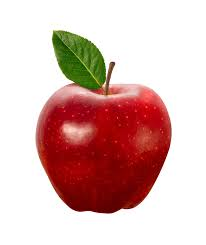
\includegraphics[width=0.4\textwidth]{results/apple_apple.jpg}}
  \hfill
  \subfloat[Apple classified as cauliflower]{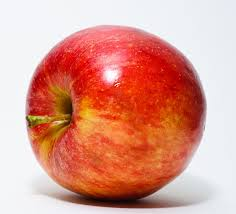
\includegraphics[width=0.4\textwidth]{results/apple_cauliflower.jpg}}
  \hfill
  \caption{Example of apple classification.}
\end{figure}

\begin{figure}[!htbp]
  \centering
  \subfloat[Broccoli classified as broccoli]{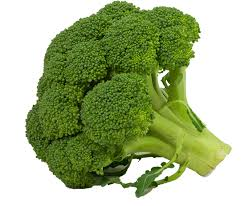
\includegraphics[width=0.4\textwidth]{results/broccoli_broccoli.jpg}}
  \hfill
  \subfloat[Broccoli classified as cauliflower]{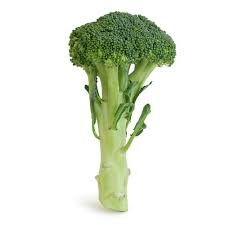
\includegraphics[width=0.4\textwidth]{results/broccoli_apple.jpg}}
  \hfill
  \caption{Example of broccoli classification.}
\end{figure}

\begin{figure}[!htbp]
  \centering
  \subfloat[Cauliflower classified as cauliflower]{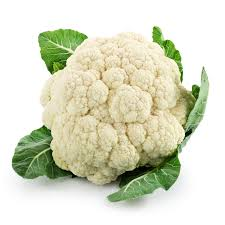
\includegraphics[width=0.4\textwidth]{results/cauliflower_cauliflower.jpg}}
  \hfill
  \subfloat[Cauliflower classified as other]{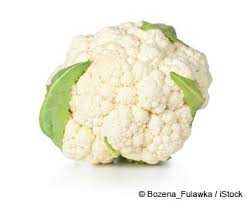
\includegraphics[width=0.4\textwidth]{results/cauliflower_other.jpg}}
  \hfill
  \caption{Example of cauliflower classification.}
\end{figure}

\begin{figure}[!htbp]
  \centering
  \subfloat[Orange classified as orange]{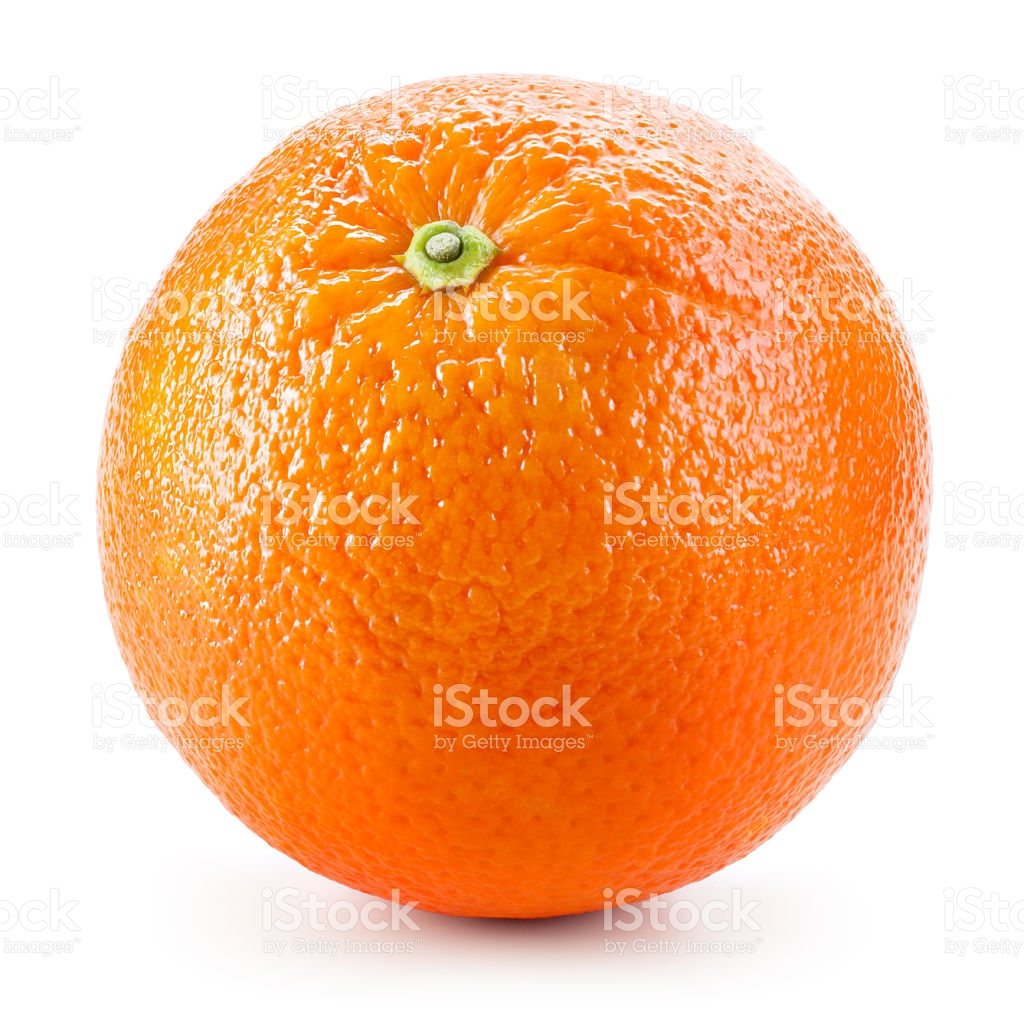
\includegraphics[width=0.4\textwidth]{results/orange_orange.jpg}}
  \hfill
  \subfloat[Orange as classified apple]{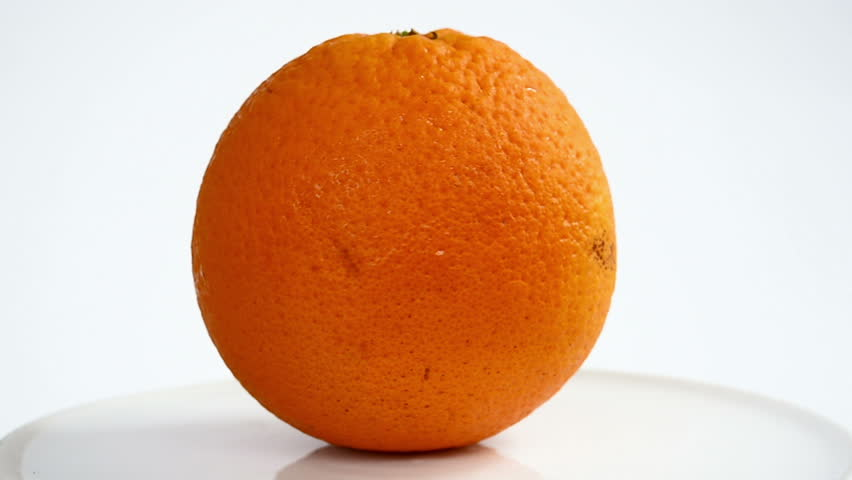
\includegraphics[width=0.4\textwidth]{results/orange_apple.jpg}}
  \hfill
  \caption{Example of orange classification.}
\end{figure}

\begin{figure}[!htbp]
  \centering
  \subfloat[Other classified as other]{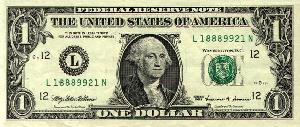
\includegraphics[width=0.4\textwidth]{results/other_other.jpg}}
  \hfill
  \subfloat[Other as classified apple]{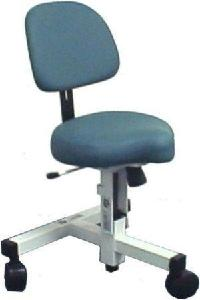
\includegraphics[width=0.4\textwidth]{results/other_apple.jpg}}
  \hfill
  \caption{Example of other classification.}
\end{figure}



\section*{Result Analysis}

ROC curve

\begin{figure}[!htbp]
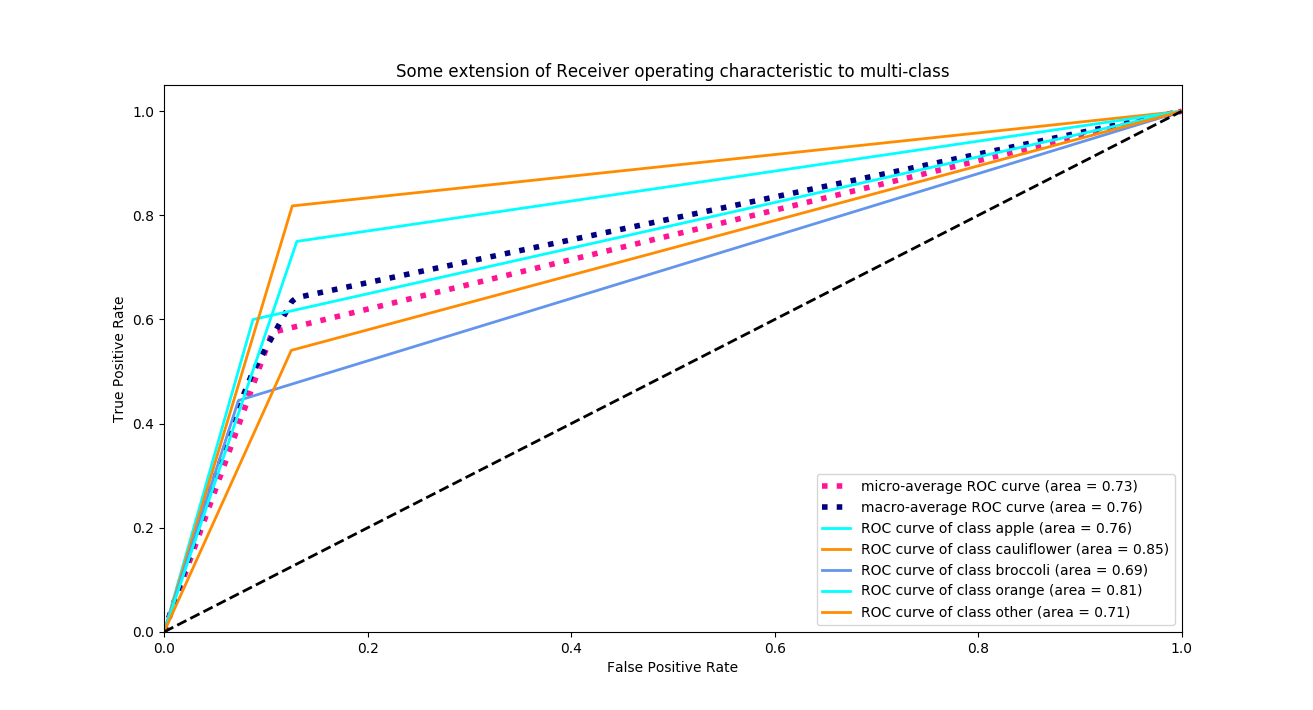
\includegraphics[scale=0.5]{results/roc.png}
\centering
\caption{ROC Curve}
\end{figure}


CMC curve is not possible to be created do due to the fact, that OpenCV's SVM implementation does not produce probabilities but only final result.


\begin{figure}[!htbp]
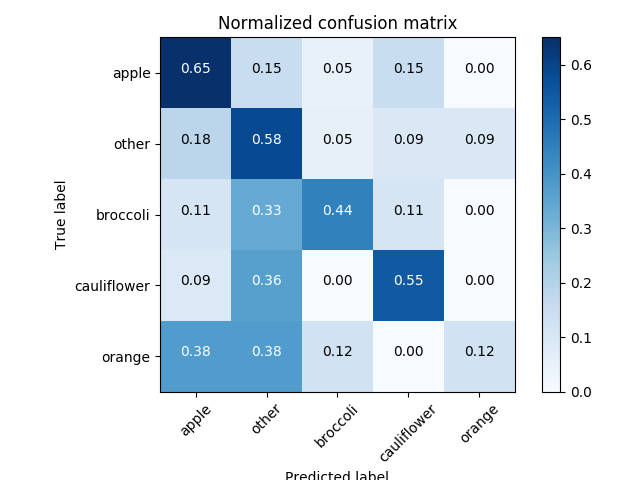
\includegraphics[scale=1]{results/confusion_matrix.png}
\centering
\caption{Confusion Matrix}
\end{figure}


As it is visible, classifier works with average precision at 73\%, recall 0.57\% and fscore 60\%. Unfortunately the overall accuracy is too low to be used in real application. It is possible that more train data with better quality would make classifier work better.


\section*{Additional Remarks}
The program was executed on two machines producing different results. In both cases classifier worked, however on the other machine results were somewhat worse, especially for orange class, for which classifying accuracy was around 10\% only. The code and data were the same and the same OpenCV version (3.3.0) was used on both computers. The reason of the difference is unknown.

\end{document}
